\documentclass{beamer}

%--------------beamer---------------
\usetheme{Warsaw}
\usecolortheme{rose}
\usefonttheme{professionalfonts}
\usepackage{tikz}
\useinnertheme{rectangles}
\useoutertheme{miniframes}
\setbeamercolor*{mini frame}{fg=black,bg=white}
\definecolor{blizzardblue}{rgb}{0.67, 0.9, 0.93}
\setbeamercolor{section in head/foot}{fg=black, bg=blizzardblue}
\definecolor{bittersweet}{rgb}{1.0, 0.44, 0.37}
\definecolor{caribbeangreen}{rgb}{0.0, 0.8, 0.6}
\definecolor{carnationpink}{rgb}{1.0, 0.65, 0.79}
\definecolor{capri}{rgb}{0.0, 0.75, 1.0}
\definecolor{green(pigment)}{rgb}{0.0, 0.65, 0.31}
\definecolor{grannysmithapple}{rgb}{0.66, 0.89, 0.63}
\defbeamertemplate{subsection in toc}{bullets}{%
  \leavevmode
  \parbox[t]{1em}{\textbullet\hfill}%
  \parbox[t]{\dimexpr\textwidth-1em\relax}{\inserttocsubsection}\par}
\defbeamertemplate{section in toc}{sections numbered roman}{%
  \leavevmode%
  \MakeUppercase{\romannumeral\inserttocsectionnumber}.\ %
  \inserttocsection\par}

\setbeamertemplate{section in toc}[sections numbered roman]
\setbeamertemplate{subsection in toc}[bullets]


%-------------packages--------------
\usepackage{graphicx} 
\usepackage{hyperref}
\usepackage{tkz-euclide,subfigure}
\usepackage{caption}
\usepackage{subcaption}
\setbeamertemplate{caption}{\raggedright\insertcaption\par}
	
\usetikzlibrary{shapes.geometric}

%------------title page-------------

\addtobeamertemplate{navigation symbols}{}{%
    \usebeamerfont{footline}%
    \usebeamercolor[fg]{footline}%
    \hspace{1em}%
    \insertframenumber/\inserttotalframenumber
}
\title{Maximum Bipartite Matching}
\author[Jahin $(2005012)$, Amim $(2005017)$ \& Tazwar $(2005020)$]
{Abrar Jahin Sarker\inst{1} \newline Abdullah  Muhammed  Amimul Ehsan\inst{2} \newline Mostafa Rifat Tazwar\inst{3}}
\institute[VFU] % (optional)
{
  \inst{1}$2005012$
  \and
  \inst{2}$2005017$
  \and
  \inst{3}$2005020$
  \and
  \inst{1,2,3}Department of Computer Science and Technology, BUET
}
\date{February 11, 2024}

\AtBeginSection
{
\begin{frame}{Outline}
    \tableofcontents[currentsection]
\end{frame}
}

\begin{document}

\begin{frame}
    \titlepage
\end{frame}

\begin{frame}{Table Of Contents}
    \tableofcontents
\end{frame}

% insert introduction

\section{Introduction}
\begin{frame}{Introduction}
    

\begin{block}{Bipartite Graph}
    A bipartite graph is one whose vertices can be split into two independent groups U,V such that every edge connects vertices of different groups.
\end{block}
\begin{alertblock}{Note}
 There can not be any edge between two vertices of U or two vertices of V .\\
     The graph is two colourable and doesn't have cycles of odd length.

\end{alertblock}

    \begin{figure}
        \centering
		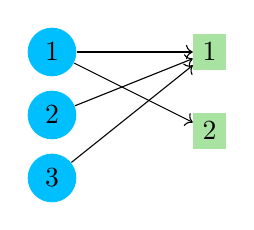
\begin{tikzpicture} 
            % 
            \node[fill=capri, circle] (b1) at (0,0) {1};
            \node[fill=capri, circle] (b2) at (0,-0.8) {2};
            \node[fill=capri, circle] (b3) at (0,-1.6) {3};
            
            % Girl
            \node[fill=grannysmithapple, rectangle] (g1) at (2,0) {1};
            \node[fill=grannysmithapple, rectangle] (g2) at (2,-1) {2};
            
            % Potential Pairs
            \draw[->] (b1) -- (g1);
            \draw[->] (b1) -- (g2);
            \draw[->] (b2) -- (g1);
            \draw[->] (b3) -- (g1);
            

        \end{tikzpicture}
        % \caption{Fig: Visualization of bipartite graph}
    \end{figure}

\end{frame}

\begin{frame}{Odd length and Even length cycle}

    \begin{figure}
    \raggedright
    \begin{minipage}[t]{0.45\linewidth}
    \centering
    
    
    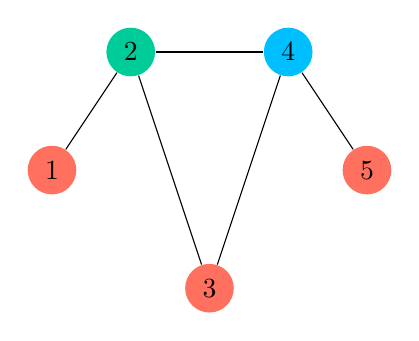
\begin{tikzpicture}
        
        
        \node[fill=bittersweet, circle] (r1) at (-0.75,0) {1} ;
        \node[fill=bittersweet, circle] (r3) at (1.25,-1.5) {3} ;
        \node[fill=bittersweet, circle] (r5) at (3.25,0) {5} ;
        \node[fill=caribbeangreen, circle] (g2) at (0.25,1.5) {2} ;
        \node[fill=capri, circle] (g4) at (2.25,1.5) {4} ;    
        
        \draw[-] (r1) -- (g2) ;
        \draw[-] (g2) -- (r3);
        \draw[-] (r3) -- (g4);
        \draw[-] (g4) -- (g2);
        \draw[-] (g4) -- (r5);
        
        
        
    \end{tikzpicture}
    \pause
    \caption*{Odd length cycle \\ Not 2 colorable  \\ \textcolor{red}{Not a bipartite graph}} \pause
    \end{minipage}%
    \hfill
    \begin{minipage}[t]{0.45\linewidth}
    \centering
    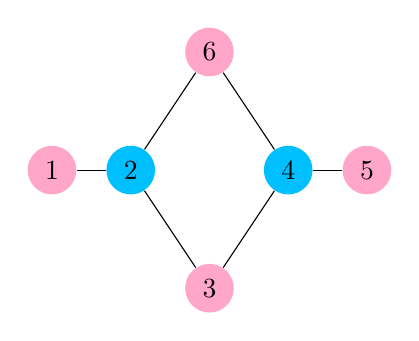
\begin{tikzpicture}
        \node[fill=carnationpink, circle] (p1) at (-0.75,0) {1} ;
        \node[fill=carnationpink, circle] (p3) at (1.25,-1.5) {3} ;
        \node[fill=carnationpink, circle] (p6) at (1.25,1.5) {6} ;
        \node[fill=carnationpink, circle] (p5) at (3.25,0) {5} ;
        \node[fill=capri, circle] (b2) at (0.25,0) {2} ;
        \node[fill=capri, circle] (b4) at (2.25,0) {4} ;    
        
        \draw[-] (p1) -- (b2) ;
        \draw[-] (b2) -- (p3);
        \draw[-] (b2) -- (p6);
        \draw[-] (b4) -- (p3);
        \draw[-] (b4) -- (p6);
        \draw[-] (b4) -- (p5);
    \end{tikzpicture} \pause
    \caption*{Even length cycle \\ 2 colorable   \\ \textcolor{green}{Bipartite graph}}
    \end{minipage}%
    \end{figure}
    
      
    \end{frame}
    


\section{Problem}

\begin{frame}{The Problem}
\begin{block}{Maximum Bipartite Matching}
     Given a bipartite graph $G = (A \cup B, E)$, find an \\ \{ $S \subseteq A \times B$ : $S$ is a matching and is as large as possible. \} \cite{kleinberg2006algorithm}
    \end{block}
\end{frame}

\section{Example}

\begin{frame}{Example}
In a picnic,there are 5 people and 5 food items.Some people express interest in some of the items.How can we satisfy maximum number of people while wasting minimum number of items?
        \pause
        \centering
		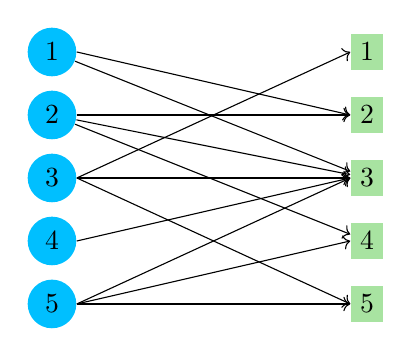
\begin{tikzpicture} 
            % 
            \node[fill=capri, circle] (p1) at (0,0) {1};
            \node[fill=capri, circle] (p2) at (0,-0.8) {2};
            \node[fill=capri, circle] (p3) at (0,-1.6) {3};
             \node[fill=capri, circle] (p4) at (0,-2.4) {4};
            \node[fill=capri, circle] (p5) at (0,-3.2) {5};
             
            
            
            % 
            \node[fill=grannysmithapple, rectangle] (f1) at (4,0) {1};
            \node[fill=grannysmithapple, rectangle] (f2) at (4,-0.8) {2};
            \node[fill=grannysmithapple, rectangle] (f3) at (4,-1.6) {3};
            \node[fill=grannysmithapple, rectangle] (f4) at (4,-2.4) {4};
            \node[fill=grannysmithapple, rectangle] (f5) at (4,-3.2) {5};
            
            % Potential Pairs
            \draw[->] (p1.east) -- (f2.west);
            \draw[->] (p1) -- (f3);
            \draw[->] (p2) -- (f2);
            \draw[->] (p2) -- (f3);
            \draw[->] (p2) -- (f4);
             \draw[->] (p3.east) -- (f1.west);
              \draw[->] (p3.east) -- (f3.west);
               \draw[->] (p3.east) -- (f5.west);
                \draw[->] (p4.east) -- (f3.west);
                  \draw[->] (p5.east) -- (f3.west);
               \draw[->] (p5.east) -- (f5.west);
                \draw[->] (p5.east) -- (f4.west);
            
            
            

        \end{tikzpicture}
    
    
\end{frame}

\section{Greedy Approach}
    \begin{frame}{Greedy Approach}
        
        Person 1 starts by taking the first available item
        \vspace{4 pt}

        \centering
		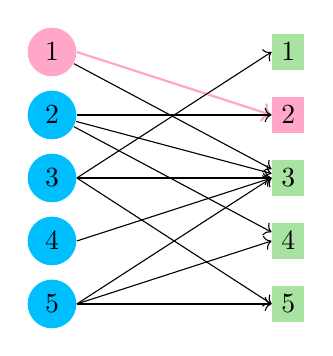
\begin{tikzpicture} 
            % 
            \node[fill=carnationpink, circle] (p1) at (0,0) {1};
            \node[fill=capri, circle] (p2) at (0,-0.8) {2};
            \node[fill=capri, circle] (p3) at (0,-1.6) {3};
             \node[fill=capri, circle] (p4) at (0,-2.4) {4};
            \node[fill=capri, circle] (p5) at (0,-3.2) {5}; 
            
            
            % 
            \node[fill=grannysmithapple, rectangle] (f1) at (3,0) {1};
            \node[fill=carnationpink, rectangle] (f2) at (3,-0.8) {2};
            \node[fill=grannysmithapple, rectangle] (f3) at (3,-1.6) {3};
            \node[fill=grannysmithapple, rectangle] (f4) at (3,-2.4) {4};
            \node[fill=grannysmithapple, rectangle] (f5) at (3,-3.2) {5};
        
            
            % Potential Pairs
           \draw[carnationpink,thick,->] (p1.east) --  (f2.west);
            \draw[->] (p1) -- (f3);
            \draw[->] (p2) -- (f2);
            \draw[->] (p2) -- (f3);
            \draw[->] (p2) -- (f4);
             \draw[->] (p3.east) -- (f1.west);
              \draw[->] (p3.east) -- (f3.west);
               \draw[->] (p3.east) -- (f5.west);
                \draw[->] (p4.east) -- (f3.west);
                  \draw[->] (p5.east) -- (f3.west);
               \draw[->] (p5.east) -- (f5.west);
                \draw[->] (p5.east) -- (f4.west);
            
            
            

        \end{tikzpicture}
    \end{frame}
    %     \begin{frame}{Greedy Approach}
        
    % Here,item 2 was already taken by person 1
    % \pause
    % \vspace{2 pt}

    %     \centering
	% 	\begin{tikzpicture} 
    %         % 
    %         \node[fill=carnationpink, circle] (p1) at (0,0) {1};
    %         \node[fill=red, circle] (p2) at (0,-0.8) {2};
    %         \node[fill=capri, circle] (p3) at (0,-1.6) {3};
    %          \node[fill=capri, circle] (p4) at (0,-2.4) {4};
    %         \node[fill=capri, circle] (p5) at (0,-3.2) {5};
             
            
            
    %         % 
    %         \node[fill=grannysmithapple, rectangle] (f1) at (4,0) {1};
    %         \node[fill=carnationpink, rectangle] (f2) at (4,-0.8) {2};
    %         \node[fill=grannysmithapple, rectangle] (f3) at (4,-1.6) {3};
    %         \node[fill=grannysmithapple, rectangle] (f4) at (4,-2.4) {4};
    %         \node[fill=grannysmithapple, rectangle] (f5) at (4,-3.2) {5};
            
    %         % Potential Pairs
    %        \draw[carnationpink,thick,->] (p1.east) --  (f2.west);
    %         \draw[->] (p1) -- (f3);
    %         \draw[red,thick,->] (p2) -- (f2);
    %         \draw[->] (p2) -- (f3);
    %         \draw[->] (p2) -- (f4);
    %          \draw[->] (p3.east) -- (f1.west);
    %           \draw[->] (p3.east) -- (f3.west);
    %            \draw[->] (p3.east) -- (f5.west);
    %             \draw[->] (p4.east) -- (f3.west);
    %               \draw[->] (p5.east) -- (f3.west);
    %            \draw[->] (p5.east) -- (f5.west);
    %             \draw[->] (p5.east) -- (f4.west);
            
            
            

    %     \end{tikzpicture}
        
    % \end{frame}
        \begin{frame}{Greedy Approach}
        
            Making item 3, the only valid choice for person 2
            \vspace{2 pt}

        \centering
		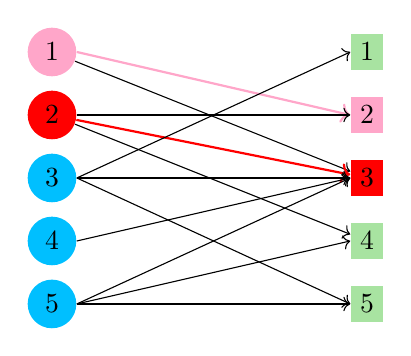
\begin{tikzpicture} 
            % 
            \node[fill=carnationpink, circle] (p1) at (0,0) {1};
            \node[fill=red, circle] (p2) at (0,-0.8) {2};
            \node[fill=capri, circle] (p3) at (0,-1.6) {3};
             \node[fill=capri, circle] (p4) at (0,-2.4) {4};
            \node[fill=capri, circle] (p5) at (0,-3.2) {5};
             
            
            
            % 
            \node[fill=grannysmithapple, rectangle] (f1) at (4,0) {1};
            \node[fill=carnationpink, rectangle] (f2) at (4,-0.8) {2};
            \node[fill=red, rectangle] (f3) at (4,-1.6) {3};
            \node[fill=grannysmithapple, rectangle] (f4) at (4,-2.4) {4};
            \node[fill=grannysmithapple, rectangle] (f5) at (4,-3.2) {5};
            
            % Potential Pairs
           \draw[carnationpink,thick,->] (p1.east) --  (f2.west);
            \draw[->] (p1) -- (f3);
            \draw[->] (p2) -- (f2);
            \draw[red,thick,->] (p2) -- (f3);
            \draw[->] (p2) -- (f4);
             \draw[->] (p3.east) -- (f1.west);
              \draw[->] (p3.east) -- (f3.west);
               \draw[->] (p3.east) -- (f5.west);
                \draw[->] (p4.east) -- (f3.west);
                  \draw[->] (p5.east) -- (f3.west);
               \draw[->] (p5.east) -- (f5.west);
                \draw[->] (p5.east) -- (f4.west);
            
            
            

        \end{tikzpicture}
        
    \end{frame}
            \begin{frame}{Greedy Approach}
        
    Here,item 1 was luckily unoccupied 
    \vspace{2 pt}

        \centering
		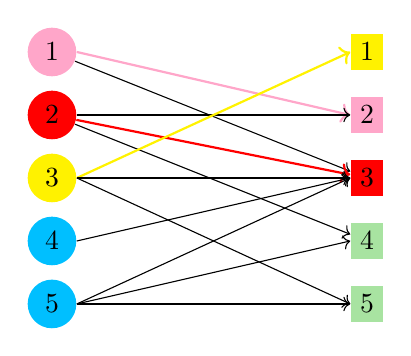
\begin{tikzpicture} 
            % 
            \node[fill=carnationpink, circle] (p1) at (0,0) {1};
            \node[fill=red, circle] (p2) at (0,-0.8) {2};
            \node[fill=yellow, circle] (p3) at (0,-1.6) {3};
             \node[fill=capri, circle] (p4) at (0,-2.4) {4};
            \node[fill=capri, circle] (p5) at (0,-3.2) {5};
             
            
            
            % 
            \node[fill=yellow, rectangle] (f1) at (4,0) {1};
            \node[fill=carnationpink, rectangle] (f2) at (4,-0.8) {2};
            \node[fill=red, rectangle] (f3) at (4,-1.6) {3};
            \node[fill=grannysmithapple, rectangle] (f4) at (4,-2.4) {4};
            \node[fill=grannysmithapple, rectangle] (f5) at (4,-3.2) {5};
            
            % Potential Pairs
           \draw[carnationpink,thick,->] (p1.east) --  (f2.west);
            \draw[->] (p1) -- (f3);
            \draw[->] (p2) -- (f2);
            \draw[red,thick,->] (p2) -- (f3);
            \draw[->] (p2) -- (f4);
             \draw[yellow,thick,->] (p3.east) -- (f1.west);
              \draw[->] (p3.east) -- (f3.west);
               \draw[->] (p3.east) -- (f5.west);
                \draw[->] (p4.east) -- (f3.west);
                  \draw[->] (p5.east) -- (f3.west);
               \draw[->] (p5.east) -- (f5.west);
                \draw[->] (p5.east) -- (f4.west);
            
            
            

        \end{tikzpicture}
        
    \end{frame}
                \begin{frame}{Greedy Approach}
        
    Here,person 4 can not have anything and person 5 got a match luckily.

    \vspace{2 pt}

        \centering
		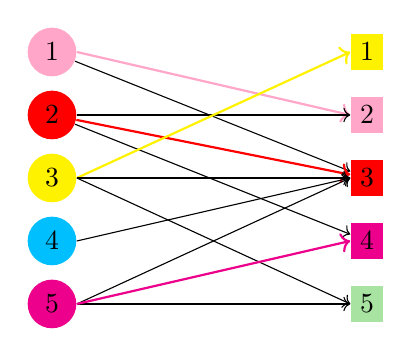
\begin{tikzpicture} 
            % 
            \node[fill=carnationpink, circle] (p1) at (0,0) {1};
            \node[fill=red, circle] (p2) at (0,-0.8) {2};
            \node[fill=yellow, circle] (p3) at (0,-1.6) {3};
             \node[fill=capri, circle] (p4) at (0,-2.4) {4};
            \node[fill=magenta, circle] (p5) at (0,-3.2) {5};
             
            
            
            % 
            \node[fill=yellow, rectangle] (f1) at (4,0) {1};
            \node[fill=carnationpink, rectangle] (f2) at (4,-0.8) {2};
            \node[fill=red, rectangle] (f3) at (4,-1.6) {3};
            \node[fill=magenta, rectangle] (f4) at (4,-2.4) {4};
            \node[fill=grannysmithapple, rectangle] (f5) at (4,-3.2) {5};
            
            % Potential Pairs
           \draw[carnationpink,thick,->] (p1.east) --  (f2.west);
            \draw[->] (p1) -- (f3);
            \draw[->] (p2) -- (f2);
            \draw[red,thick,->] (p2) -- (f3);
            \draw[->] (p2) -- (f4);
             \draw[yellow,thick,->] (p3.east) -- (f1.west);
              \draw[->] (p3.east) -- (f3.west);
               \draw[->] (p3.east) -- (f5.west);
                \draw[->] (p4.east) -- (f3.west);
                  \draw[->] (p5.east) -- (f3.west);
               \draw[->] (p5.east) -- (f5.west);
                \draw[magenta,thick,->] (p5.east) -- (f4.west);
            
            
            

        \end{tikzpicture}
        \pause
        \\
        We could only satisfy four guests.One guest is unhappy.
        
    \end{frame}
\section{Reduction}
\begin{frame}{Approach to solve }
    \begin{columns}[T]
        \begin{column}{0.4\textwidth}
            % Text column
            \begin{itemize}
                \item Given an instance of bipartite matching
                \pause
                \item Reduce it to Max Flow Problem.
                \pause
                \item 
Where the solution to the
network 
flow problem can
easily be used to find the
solution to the bipartite
matching.
            \end{itemize}
        \end{column}
        
        \begin{column}{0.5\textwidth}
            % Flowchart column
            \begin{figure}
                \centering
		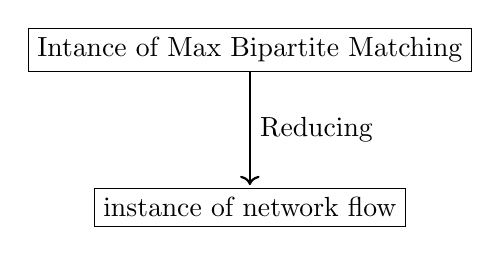
\begin{tikzpicture} [shorten >=1pt,node distance=2cm,auto]
                    % Nodes
                    \node[draw,rectangle] (A1) {Intance of Max Bipartite Matching};
                    \node[draw,rectangle] (B5) [below of=A1] {instance of network flow};
                
                    % Arrow
                    \draw[black,thick,->] (A1.south) -- node[midway, right] {Reducing} (B5.north);
                \end{tikzpicture}
            \end{figure}
        \end{column}
    \end{columns}
\end{frame}
% \begin{frame}{Reducing to Network Flow Problem}
% \textbf{Approach: }\\


% \begin{block}{}
%     % \begin{itemize}
%     %     \item Make all the edges directed if not and add 0 flow and 1 capacity for all edges.Expressed as 0/1 in Flow/Capacity format
%     %     \pause
%         % \item Add two new nodes: 
%         % \pause
%         % \begin{enumerate}
%         %     \item Source(S)
%         %     \item Destination(t)
%         % \end{enumerate}
%     %     \pause
%     %     \item 
%     %     Add nodes from source to person with flow/capacity=0/1.
%     %     \pause
%     %     \item 
%     %     Add nodes from food items to destination with 0 flow and 1 capacity
%     %     \pause
%     %     \item After applying network flow algorithm, flow \textgreater{}     0 between the pairs indicates a matching.
        
%     % \end{itemize}
    
% \end{frame}

% \begin{frame}{Reduced to Network Flow}


%         \centering
% 		\begin{tikzpicture} 
%             \node[fill=yellow,rectangle](s) at (-3,-1.6) {S};
%             \node[fill=bittersweet,rectangle](t) at (7,-1.6) {t};

%             \draw[->](s.east)--node[right,above,font=\small]{0/1} (p1.west);
%             \draw[->](s.east)--node[midway,right,font=\small]{0/1} (p2.west);
%             \draw[->](s.east)--node[midway,left,font=\small]{0/1} (p3.west);
%             \draw[->](s.east)--node[midway,right,font=\small]{0/1} (p4.west);
%             \draw[->](s.east)--node[midway,left,font=\small]{0/1} (p5.west);


%             \draw[->](f1.east)--node[midway,above,font=\small]{0/1} (t.west);
%             \draw[->](f2.east)--node[midway,left,font=\small]{0/1} (t.west);
%             \draw[->](f3.east)--node[left,right,font=\small]{0/1} (t.west);
%             \draw[->](f4.east)--node[left,right,font=\small]{0/1} (t.west);
%             \draw[->](f5.east)--node[left,right,font=\small]{0/1} (t.west);


            
%             \node[fill=capri, circle] (p1) at (0,0) {1};
%             \node[fill=capri, circle] (p2) at (0,-0.8) {2};
%             \node[fill=capri, circle] (p3) at (0,-1.6) {3};
%              \node[fill=capri, circle] (p4) at (0,-2.4) {4};
%             \node[fill=capri, circle] (p5) at (0,-3.2) {5};
             
            
            
            
%             \node[fill=grannysmithapple, rectangle] (f1) at (4,0) {1};
%             \node[fill=grannysmithapple, rectangle] (f2) at (4,-0.8) {2};
%             \node[fill=grannysmithapple, rectangle] (f3) at (4,-1.6) {3};
%             \node[fill=grannysmithapple, rectangle] (f4) at (4,-2.4) {4};
%             \node[fill=grannysmithapple, rectangle] (f5) at (4,-3.2) {5};
            
%             % Potential Pairs
%             \draw[->] (p1.east)--node[midway,above,font=\small]{0/1}  (f2.west);
%             \draw[->] (p1) -- node[near start,left,font=\small]{0/1}  (f3);
%             \draw[->] (p2) -- node[near end,left,font=\small]{0/1}  (f2);
%             \draw[->] (p2) -- node[midway,right,font=\small]{0/1}  (f3);
%             \draw[->] (p2) -- node[near end,right,font=\small]{0/1} (f4);
%              \draw[->] (p3.east) -- node[near end,right,font=\small]{0/1}  (f1.west);
%               \draw[->] (p3.east) -- node[near end,right,font=\small]{0/1}  (f3.west);
%                \draw[->] (p3.east) -- node[near end,right,font=\small]{0/1}  (f5.west);
%                 \draw[->] (p4.east) -- node[near start,above,font=\small]{0/1}  (f3.west);
%                   \draw[->] (p5.east) -- node[near start,above,font=\small]{0/1} (f3.west);
%                \draw[->] (p5.east) -- node[near end,below,font=\small]{0/1}  (f5.west);
%                 \draw[->] (p5.east) -- node[near end,above,font=\small]{0/1} (f4.west);
            
            
            

%         \end{tikzpicture}
    
    
% \end{frame}
\begin{frame}{Reduction}
    \begin{block}{Step 1}
            Make all the edges directed if not and add 0 flow and 1 capacity for all edges.Expressed as 0/1 in Flow/Capacity format
        \end{block}
        \centering
        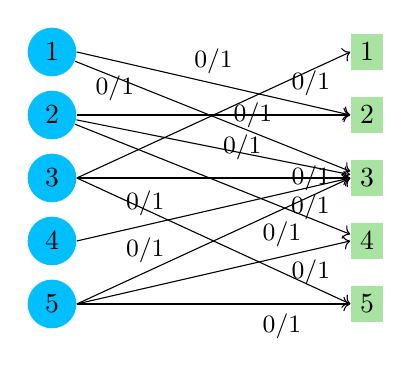
\begin{tikzpicture} 
               
    
    
                
                \node[fill=capri, circle] (p1) at (0,0) {1};
                \node[fill=capri, circle] (p2) at (0,-0.8) {2};
                \node[fill=capri, circle] (p3) at (0,-1.6) {3};
                 \node[fill=capri, circle] (p4) at (0,-2.4) {4};
                \node[fill=capri, circle] (p5) at (0,-3.2) {5};
                 
                
                
                
                \node[fill=grannysmithapple, rectangle] (f1) at (4,0) {1};
                \node[fill=grannysmithapple, rectangle] (f2) at (4,-0.8) {2};
                \node[fill=grannysmithapple, rectangle] (f3) at (4,-1.6) {3};
                \node[fill=grannysmithapple, rectangle] (f4) at (4,-2.4) {4};
                \node[fill=grannysmithapple, rectangle] (f5) at (4,-3.2) {5};
                
                % Potential Pairs
                \draw[->] (p1.east)--node[midway,above,font=\small]{0/1}  (f2.west);
                \draw[->] (p1) -- node[near start,left,font=\small]{0/1}  (f3);
                \draw[->] (p2) -- node[near end,left,font=\small]{0/1}  (f2);
                \draw[->] (p2) -- node[midway,right,font=\small]{0/1}  (f3);
                \draw[->] (p2) -- node[near end,right,font=\small]{0/1} (f4);
                 \draw[->] (p3.east) -- node[near end,right,font=\small]{0/1}  (f1.west);
                  \draw[->] (p3.east) -- node[near end,right,font=\small]{0/1}  (f3.west);
                   \draw[->] (p3.east) -- node[near end,right,font=\small]{0/1}  (f5.west);
                    \draw[->] (p4.east) -- node[near start,above,font=\small]{0/1}  (f3.west);
                      \draw[->] (p5.east) -- node[near start,above,font=\small]{0/1} (f3.west);
                   \draw[->] (p5.east) -- node[near end,below,font=\small]{0/1}  (f5.west);
                    \draw[->] (p5.east) -- node[near end,above,font=\small]{0/1} (f4.west);
                
                
                
    
            \end{tikzpicture}
        
    \end{frame}
    \begin{frame}{Reduction}
    \begin{block}{Step 2}
                  Add two new nodes: 
            
            \begin{enumerate}
                \item Source(S)
                \item Destination(t)
            \end{enumerate}
        \end{block}
        \centering
        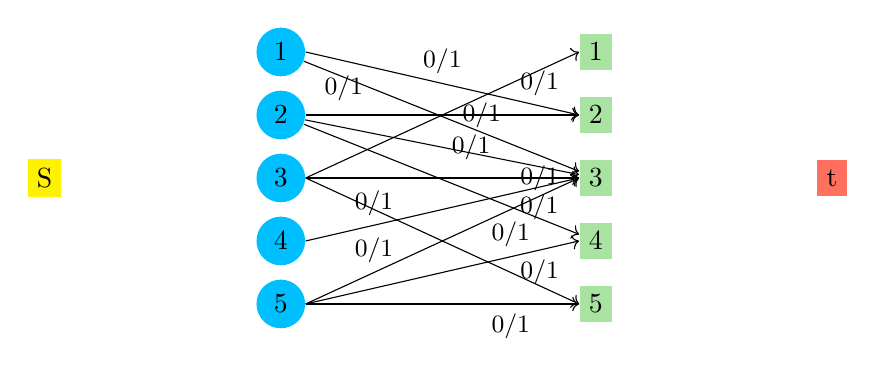
\begin{tikzpicture} 
               
    
                            \node[fill=yellow,rectangle](s) at (-3,-1.6) {S};
                \node[fill=bittersweet,rectangle](t) at (7,-1.6) {t};
                
                \node[fill=capri, circle] (p1) at (0,0) {1};
                \node[fill=capri, circle] (p2) at (0,-0.8) {2};
                \node[fill=capri, circle] (p3) at (0,-1.6) {3};
                 \node[fill=capri, circle] (p4) at (0,-2.4) {4};
                \node[fill=capri, circle] (p5) at (0,-3.2) {5};
                 
                
                
                
                \node[fill=grannysmithapple, rectangle] (f1) at (4,0) {1};
                \node[fill=grannysmithapple, rectangle] (f2) at (4,-0.8) {2};
                \node[fill=grannysmithapple, rectangle] (f3) at (4,-1.6) {3};
                \node[fill=grannysmithapple, rectangle] (f4) at (4,-2.4) {4};
                \node[fill=grannysmithapple, rectangle] (f5) at (4,-3.2) {5};
                
                % Potential Pairs
                \draw[->] (p1.east)--node[midway,above,font=\small]{0/1}  (f2.west);
                \draw[->] (p1) -- node[near start,left,font=\small]{0/1}  (f3);
                \draw[->] (p2) -- node[near end,left,font=\small]{0/1}  (f2);
                \draw[->] (p2) -- node[midway,right,font=\small]{0/1}  (f3);
                \draw[->] (p2) -- node[near end,right,font=\small]{0/1} (f4);
                 \draw[->] (p3.east) -- node[near end,right,font=\small]{0/1}  (f1.west);
                  \draw[->] (p3.east) -- node[near end,right,font=\small]{0/1}  (f3.west);
                   \draw[->] (p3.east) -- node[near end,right,font=\small]{0/1}  (f5.west);
                    \draw[->] (p4.east) -- node[near start,above,font=\small]{0/1}  (f3.west);
                      \draw[->] (p5.east) -- node[near start,above,font=\small]{0/1} (f3.west);
                   \draw[->] (p5.east) -- node[near end,below,font=\small]{0/1}  (f5.west);
                    \draw[->] (p5.east) -- node[near end,above,font=\small]{0/1} (f4.west);
                
                
                
    
            \end{tikzpicture}
        
    \end{frame}
    \begin{frame}{Reduction}
    \begin{block}{Step 3}
                Add nodes from source to person with flow/capacity=0/1.
        \end{block}
        \begin{tikzpicture} 
               
    
                            \node[fill=yellow,rectangle](s) at (-3,-1.6) {S};
                \node[fill=bittersweet,rectangle](t) at (7,-1.6) {t};
    
    
                \draw[red,->](s.east)--node[right,above,font=\small]{0/1} (p1.west);
                \draw[red,->](s.east)--node[midway,right,font=\small]{0/1} (p2.west);
                \draw[red,->](s.east)--node[midway,left,font=\small]{0/1} (p3.west);
                \draw[red,->](s.east)--node[midway,right,font=\small]{0/1} (p4.west);
                \draw[red,->](s.east)--node[midway,left,font=\small]{0/1} (p5.west);
    
    
                
                
                \node[fill=capri, circle] (p1) at (0,0) {1};
                \node[fill=capri, circle] (p2) at (0,-0.8) {2};
                \node[fill=capri, circle] (p3) at (0,-1.6) {3};
                 \node[fill=capri, circle] (p4) at (0,-2.4) {4};
                \node[fill=capri, circle] (p5) at (0,-3.2) {5};
                 
                
                
                
                \node[fill=grannysmithapple, rectangle] (f1) at (4,0) {1};
                \node[fill=grannysmithapple, rectangle] (f2) at (4,-0.8) {2};
                \node[fill=grannysmithapple, rectangle] (f3) at (4,-1.6) {3};
                \node[fill=grannysmithapple, rectangle] (f4) at (4,-2.4) {4};
                \node[fill=grannysmithapple, rectangle] (f5) at (4,-3.2) {5};
                
                % Potential Pairs
                \draw[->] (p1.east)--node[midway,above,font=\small]{0/1}  (f2.west);
                \draw[->] (p1) -- node[near start,left,font=\small]{0/1}  (f3);
                \draw[->] (p2) -- node[near end,left,font=\small]{0/1}  (f2);
                \draw[->] (p2) -- node[midway,right,font=\small]{0/1}  (f3);
                \draw[->] (p2) -- node[near end,right,font=\small]{0/1} (f4);
                 \draw[->] (p3.east) -- node[near end,right,font=\small]{0/1}  (f1.west);
                  \draw[->] (p3.east) -- node[near end,right,font=\small]{0/1}  (f3.west);
                   \draw[->] (p3.east) -- node[near end,right,font=\small]{0/1}  (f5.west);
                    \draw[->] (p4.east) -- node[near start,above,font=\small]{0/1}  (f3.west);
                      \draw[->] (p5.east) -- node[near start,above,font=\small]{0/1} (f3.west);
                   \draw[->] (p5.east) -- node[near end,below,font=\small]{0/1}  (f5.west);
                    \draw[->] (p5.east) -- node[near end,above,font=\small]{0/1} (f4.west);
                
                
                
    
            \end{tikzpicture}
        
    \end{frame}
    \begin{frame}{Reduction}
    \begin{block}{Step 4}
                Add nodes from food items to destination with 0 flow and 1 capacity
        \end{block}
        \centering
        \begin{tikzpicture} 
               
    
                            \node[fill=yellow,rectangle](s) at (-3,-1.6) {S};
                \node[fill=bittersweet,rectangle](t) at (7,-1.6) {t};
    
    
            
                \draw[->](s.east)--node[right,above,font=\small]{0/1} (p1.west);
                \draw[->](s.east)--node[midway,right,font=\small]{0/1} (p2.west);
                \draw[->](s.east)--node[midway,left,font=\small]{0/1} (p3.west);
                \draw[->](s.east)--node[midway,right,font=\small]{0/1} (p4.west);
                \draw[->](s.east)--node[midway,left,font=\small]{0/1} (p5.west);
    
    
                \draw[red,->](f1.east)--node[midway,above,font=\small]{0/1} (t.west);
                \draw[red,->](f2.east)--node[midway,left,font=\small]{0/1} (t.west);
                \draw[red,->](f3.east)--node[left,right,font=\small]{0/1} (t.west);
                \draw[red,->](f4.east)--node[left,right,font=\small]{0/1} (t.west);
                \draw[red,->](f5.east)--node[left,right,font=\small]{0/1} (t.west);
    
    
                
                
                \node[fill=capri, circle] (p1) at (0,0) {1};
                \node[fill=capri, circle] (p2) at (0,-0.8) {2};
                \node[fill=capri, circle] (p3) at (0,-1.6) {3};
                 \node[fill=capri, circle] (p4) at (0,-2.4) {4};
                \node[fill=capri, circle] (p5) at (0,-3.2) {5};
                 
                
                
                
                \node[fill=grannysmithapple, rectangle] (f1) at (4,0) {1};
                \node[fill=grannysmithapple, rectangle] (f2) at (4,-0.8) {2};
                \node[fill=grannysmithapple, rectangle] (f3) at (4,-1.6) {3};
                \node[fill=grannysmithapple, rectangle] (f4) at (4,-2.4) {4};
                \node[fill=grannysmithapple, rectangle] (f5) at (4,-3.2) {5};
                
                % Potential Pairs
                \draw[->] (p1.east)--node[midway,above,font=\small]{0/1}  (f2.west);
                \draw[->] (p1) -- node[near start,left,font=\small]{0/1}  (f3);
                \draw[->] (p2) -- node[near end,left,font=\small]{0/1}  (f2);
                \draw[->] (p2) -- node[midway,right,font=\small]{0/1}  (f3);
                \draw[->] (p2) -- node[near end,right,font=\small]{0/1} (f4);
                 \draw[->] (p3.east) -- node[near end,right,font=\small]{0/1}  (f1.west);
                  \draw[->] (p3.east) -- node[near end,right,font=\small]{0/1}  (f3.west);
                   \draw[->] (p3.east) -- node[near end,right,font=\small]{0/1}  (f5.west);
                    \draw[->] (p4.east) -- node[near start,above,font=\small]{0/1}  (f3.west);
                      \draw[->] (p5.east) -- node[near start,above,font=\small]{0/1} (f3.west);
                   \draw[->] (p5.east) -- node[near end,below,font=\small]{0/1}  (f5.west);
                    \draw[->] (p5.east) -- node[near end,above,font=\small]{0/1} (f4.west);
                
                
                
    
            \end{tikzpicture}
        
    \end{frame}
    \begin{frame}{Reduced to Network Flow Problem}
    \begin{block}{Finally}
    It is reduced to a network flow problem where we have to apply
     network flow algorithm.Here, flow \textgreater{}   0 between the pairs indicates a matching.
    \end{block}
         \centering
            \begin{tikzpicture} 
                \node[fill=yellow,rectangle](s) at (-3,-1.6) {S};
                \node[fill=bittersweet,rectangle](t) at (7,-1.6) {t};
    
                \draw[->](s.east)--node[right,above,font=\small]{0/1} (p1.west);
                \draw[->](s.east)--node[midway,right,font=\small]{0/1} (p2.west);
                \draw[->](s.east)--node[midway,left,font=\small]{0/1} (p3.west);
                \draw[->](s.east)--node[midway,right,font=\small]{0/1} (p4.west);
                \draw[->](s.east)--node[midway,left,font=\small]{0/1} (p5.west);
    
    
                \draw[->](f1.east)--node[midway,above,font=\small]{0/1} (t.west);
                \draw[->](f2.east)--node[midway,left,font=\small]{0/1} (t.west);
                \draw[->](f3.east)--node[left,right,font=\small]{0/1} (t.west);
                \draw[->](f4.east)--node[left,right,font=\small]{0/1} (t.west);
                \draw[->](f5.east)--node[left,right,font=\small]{0/1} (t.west);
    
    
                
                \node[fill=capri, circle] (p1) at (0,0) {1};
                \node[fill=capri, circle] (p2) at (0,-0.8) {2};
                \node[fill=capri, circle] (p3) at (0,-1.6) {3};
                 \node[fill=capri, circle] (p4) at (0,-2.4) {4};
                \node[fill=capri, circle] (p5) at (0,-3.2) {5};
                 
                
                
                
                \node[fill=grannysmithapple, rectangle] (f1) at (4,0) {1};
                \node[fill=grannysmithapple, rectangle] (f2) at (4,-0.8) {2};
                \node[fill=grannysmithapple, rectangle] (f3) at (4,-1.6) {3};
                \node[fill=grannysmithapple, rectangle] (f4) at (4,-2.4) {4};
                \node[fill=grannysmithapple, rectangle] (f5) at (4,-3.2) {5};
                
                % Potential Pairs
                \draw[->] (p1.east)--node[midway,above,font=\small]{0/1}  (f2.west);
                \draw[->] (p1) -- node[near start,left,font=\small]{0/1}  (f3);
                \draw[->] (p2) -- node[near end,left,font=\small]{0/1}  (f2);
                \draw[->] (p2) -- node[midway,right,font=\small]{0/1}  (f3);
                \draw[->] (p2) -- node[near end,right,font=\small]{0/1} (f4);
                 \draw[->] (p3.east) -- node[near end,right,font=\small]{0/1}  (f1.west);
                  \draw[->] (p3.east) -- node[near end,right,font=\small]{0/1}  (f3.west);
                   \draw[->] (p3.east) -- node[near end,right,font=\small]{0/1}  (f5.west);
                    \draw[->] (p4.east) -- node[near start,above,font=\small]{0/1}  (f3.west);
                      \draw[->] (p5.east) -- node[near start,above,font=\small]{0/1} (f3.west);
                   \draw[->] (p5.east) -- node[near end,below,font=\small]{0/1}  (f5.west);
                    \draw[->] (p5.east) -- node[near end,above,font=\small]{0/1} (f4.west);
                
                
                
    
            \end{tikzpicture}
        
    \end{frame}

\begin{frame}{Edmonds-Karp Algorithm to Solve Network Flow Problem}
        \begin{itemize}
        \item Initialize flow $f(u,v) = 0$ for all edges $(u,v)$ in the graph.
        \item Repeat the following steps until no augmenting paths can be found:
        \begin{itemize}
            \item Use BFS to find the shortest augmenting path from source to sink.
            \item If no augmenting path is found, terminate.
            \item Let $P$ be the augmenting path found by BFS.
            \item Let $cf(P)$ be the minimum residual capacity along path $P$.
            \item For each edge $(u,v)$ in $P$:
            \begin{itemize}
                \item Update flow $f(u,v) = f(u,v) + cf(P)$.
                \item Update flow $f(v,u) = f(v,u) - cf(P)$ for the reverse edge.
            \end{itemize}
        \end{itemize}
        \item The value of the maximum flow is the sum of flow values leaving the source.
    \end{itemize}

\end{frame}
\section{Solution}
\begin{frame}{Solution to Network Flow Problem}


        \centering
		\begin{tikzpicture} 
            \node[fill=yellow,rectangle](s) at (-3,-1.6) {S};
            \node[fill=bittersweet,rectangle](t) at (7,-1.6) {t};

            \draw[brown,->](s.east)--node[right,above,font=\small]{1/1} (p1.west);
            \draw[->](s.east)--node[midway,right,font=\small]{0/1} (p2.west);
            \draw[->](s.east)--node[midway,left,font=\small]{0/1} (p3.west);
            \draw[->](s.east)--node[midway,right,font=\small]{0/1} (p4.west);
            \draw[->](s.east)--node[midway,left,font=\small]{0/1} (p5.west);


            \draw[->](f1.east)--node[midway,above,font=\small]{0/1} (t.west);
            \draw[brown,->](f2.east)--node[midway,left,font=\small]{1/1} (t.west);
            \draw[->](f3.east)--node[left,right,font=\small]{0/1} (t.west);
            \draw[->](f4.east)--node[left,right,font=\small]{0/1} (t.west);
            \draw[->](f5.east)--node[left,right,font=\small]{0/1} (t.west);


            
            \node[fill=capri, circle] (p1) at (0,0) {1};
            \node[fill=capri, circle] (p2) at (0,-0.8) {2};
            \node[fill=capri, circle] (p3) at (0,-1.6) {3};
             \node[fill=capri, circle] (p4) at (0,-2.4) {4};
            \node[fill=capri, circle] (p5) at (0,-3.2) {5};
             
            
            
            
            \node[fill=grannysmithapple, rectangle] (f1) at (4,0) {1};
            \node[fill=grannysmithapple, rectangle] (f2) at (4,-0.8) {2};
            \node[fill=grannysmithapple, rectangle] (f3) at (4,-1.6) {3};
            \node[fill=grannysmithapple, rectangle] (f4) at (4,-2.4) {4};
            \node[fill=grannysmithapple, rectangle] (f5) at (4,-3.2) {5};
            
            % Potential Pairs
            \draw[brown,->] (p1.east)--node[midway,above,font=\small]{1/1}  (f2.west);
            \draw[->] (p1) -- node[near start,left,font=\small]{0/1}  (f3);
            \draw[->] (p2) -- node[near end,left,font=\small]{0/1}  (f2);
            \draw[->] (p2) -- node[midway,right,font=\small]{0/1}  (f3);
            \draw[->] (p2) -- node[near end,right,font=\small]{0/1} (f4);
             \draw[->] (p3.east) -- node[near end,right,font=\small]{0/1}  (f1.west);
              \draw[->] (p3.east) -- node[near end,right,font=\small]{0/1}  (f3.west);
               \draw[->] (p3.east) -- node[near end,right,font=\small]{0/1}  (f5.west);
                \draw[->] (p4.east) -- node[near start,above,font=\small]{0/1}  (f3.west);
                  \draw[->] (p5.east) -- node[near start,above,font=\small]{0/1} (f3.west);
               \draw[->] (p5.east) -- node[near end,below,font=\small]{0/1}  (f5.west);
                \draw[->] (p5.east) -- node[near end,above,font=\small]{0/1} (f4.west);
            
            
            

        \end{tikzpicture}
    
    
\end{frame}

\begin{frame}{Solution to Network Flow Problem}


        \centering
		\begin{tikzpicture} 
            \node[fill=yellow,rectangle](s) at (-3,-1.6) {S};
            \node[fill=bittersweet,rectangle](t) at (7,-1.6) {t};

            \draw[brown,->](s.east)--node[right,above,font=\small]{1/1} (p1.west);
            \draw[brown,->](s.east)--node[midway,right,font=\small]{1/1} (p2.west);
            \draw[->](s.east)--node[midway,left,font=\small]{0/1} (p3.west);
            \draw[->](s.east)--node[midway,right,font=\small]{0/1} (p4.west);
            \draw[->](s.east)--node[midway,left,font=\small]{0/1} (p5.west);


            \draw[->](f1.east)--node[midway,above,font=\small]{0/1} (t.west);
            \draw[brown,->](f2.east)--node[midway,left,font=\small]{1/1} (t.west);
            \draw[->](f3.east)--node[left,right,font=\small]{0/1} (t.west);
            \draw[brown,->](f4.east)--node[left,right,font=\small]{1/1} (t.west);
            \draw[->](f5.east)--node[left,right,font=\small]{0/1} (t.west);


            
            \node[fill=capri, circle] (p1) at (0,0) {1};
            \node[fill=capri, circle] (p2) at (0,-0.8) {2};
            \node[fill=capri, circle] (p3) at (0,-1.6) {3};
             \node[fill=capri, circle] (p4) at (0,-2.4) {4};
            \node[fill=capri, circle] (p5) at (0,-3.2) {5};
             
            
            
            
            \node[fill=grannysmithapple, rectangle] (f1) at (4,0) {1};
            \node[fill=grannysmithapple, rectangle] (f2) at (4,-0.8) {2};
            \node[fill=grannysmithapple, rectangle] (f3) at (4,-1.6) {3};
            \node[fill=grannysmithapple, rectangle] (f4) at (4,-2.4) {4};
            \node[fill=grannysmithapple, rectangle] (f5) at (4,-3.2) {5};
            
            % Potential Pairs
            \draw[brown,->] (p1.east)--node[midway,above,font=\small]{1/1}  (f2.west);
            \draw[->] (p1) -- node[near start,left,font=\small]{0/1}  (f3);
            \draw[->] (p2) -- node[near end,left,font=\small]{0/1}  (f2);
            \draw[->] (p2) -- node[midway,right,font=\small]{0/1}  (f3);
            \draw[brown,->] (p2) -- node[near end,right,font=\small]{1/1} (f4);
             \draw[->] (p3.east) -- node[near end,right,font=\small]{0/1}  (f1.west);
              \draw[->] (p3.east) -- node[near end,right,font=\small]{0/1}  (f3.west);
               \draw[->] (p3.east) -- node[near end,right,font=\small]{0/1}  (f5.west);
                \draw[->] (p4.east) -- node[near start,above,font=\small]{0/1}  (f3.west);
                  \draw[->] (p5.east) -- node[near start,above,font=\small]{0/1} (f3.west);
               \draw[->] (p5.east) -- node[near end,below,font=\small]{0/1}  (f5.west);
                \draw[->] (p5.east) -- node[near end,above,font=\small]{0/1} (f4.west);
            
            
            

        \end{tikzpicture}
    
    
\end{frame}

\begin{frame}{Solution to Network Flow Problem}


        \centering
		\begin{tikzpicture} 
            \node[fill=yellow,rectangle](s) at (-3,-1.6) {S};
            \node[fill=bittersweet,rectangle](t) at (7,-1.6) {t};

            \draw[brown,->](s.east)--node[right,above,font=\small]{1/1} (p1.west);
            \draw[brown,->](s.east)--node[midway,right,font=\small]{1/1} (p2.west);
            \draw[brown,->](s.east)--node[midway,left,font=\small]{1/1} (p3.west);
            \draw[->](s.east)--node[midway,right,font=\small]{0/1} (p4.west);
            \draw[->](s.east)--node[midway,left,font=\small]{0/1} (p5.west);


            \draw[brown,->](f1.east)--node[midway,above,font=\small]{1/1} (t.west);
            \draw[brown,->](f2.east)--node[midway,left,font=\small]{1/1} (t.west);
            \draw[->](f3.east)--node[left,right,font=\small]{0/1} (t.west);
            \draw[brown,->](f4.east)--node[left,right,font=\small]{1/1} (t.west);
            \draw[->](f5.east)--node[left,right,font=\small]{0/1} (t.west);


            
            \node[fill=capri, circle] (p1) at (0,0) {1};
            \node[fill=capri, circle] (p2) at (0,-0.8) {2};
            \node[fill=capri, circle] (p3) at (0,-1.6) {3};
             \node[fill=capri, circle] (p4) at (0,-2.4) {4};
            \node[fill=capri, circle] (p5) at (0,-3.2) {5};
             
            
            
            
            \node[fill=grannysmithapple, rectangle] (f1) at (4,0) {1};
            \node[fill=grannysmithapple, rectangle] (f2) at (4,-0.8) {2};
            \node[fill=grannysmithapple, rectangle] (f3) at (4,-1.6) {3};
            \node[fill=grannysmithapple, rectangle] (f4) at (4,-2.4) {4};
            \node[fill=grannysmithapple, rectangle] (f5) at (4,-3.2) {5};
            
            % Potential Pairs
            \draw[brown,->] (p1.east)--node[midway,above,font=\small]{1/1}  (f2.west);
            \draw[->] (p1) -- node[near start,left,font=\small]{0/1}  (f3);
            \draw[->] (p2) -- node[near end,left,font=\small]{0/1}  (f2);
            \draw[->] (p2) -- node[midway,right,font=\small]{0/1}  (f3);
            \draw[brown,->] (p2) -- node[near end,right,font=\small]{1/1} (f4);
             \draw[brown,->] (p3.east) -- node[near end,right,font=\small]{1/1}  (f1.west);
              \draw[->] (p3.east) -- node[near end,right,font=\small]{0/1}  (f3.west);
               \draw[->] (p3.east) -- node[near end,right,font=\small]{0/1}  (f5.west);
                \draw[->] (p4.east) -- node[near start,above,font=\small]{0/1}  (f3.west);
                  \draw[->] (p5.east) -- node[near start,above,font=\small]{0/1} (f3.west);
               \draw[->] (p5.east) -- node[near end,below,font=\small]{0/1}  (f5.west);
                \draw[->] (p5.east) -- node[near end,above,font=\small]{0/1} (f4.west);
            
            
            

        \end{tikzpicture}
    
    
\end{frame}

\begin{frame}{Solution to Network Flow Problem}


        \centering
		\begin{tikzpicture} 
            \node[fill=yellow,rectangle](s) at (-3,-1.6) {S};
            \node[fill=bittersweet,rectangle](t) at (7,-1.6) {t};

            \draw[brown,->](s.east)--node[right,above,font=\small]{1/1} (p1.west);
            \draw[brown,->](s.east)--node[midway,right,font=\small]{1/1} (p2.west);
            \draw[brown,->](s.east)--node[midway,left,font=\small]{1/1} (p3.west);
            \draw[brown,->](s.east)--node[midway,right,font=\small]{1/1} (p4.west);
            \draw[->](s.east)--node[midway,left,font=\small]{0/1} (p5.west);


            \draw[brown,->](f1.east)--node[midway,above,font=\small]{1/1} (t.west);
            \draw[brown,->](f2.east)--node[midway,left,font=\small]{1/1} (t.west);
            \draw[brown,->](f3.east)--node[left,right,font=\small]{1/1} (t.west);
            \draw[brown,->](f4.east)--node[left,right,font=\small]{1/1} (t.west);
            \draw[->](f5.east)--node[left,right,font=\small]{0/1} (t.west);


            
            \node[fill=capri, circle] (p1) at (0,0) {1};
            \node[fill=capri, circle] (p2) at (0,-0.8) {2};
            \node[fill=capri, circle] (p3) at (0,-1.6) {3};
             \node[fill=capri, circle] (p4) at (0,-2.4) {4};
            \node[fill=capri, circle] (p5) at (0,-3.2) {5};
             
            
            
            
            \node[fill=grannysmithapple, rectangle] (f1) at (4,0) {1};
            \node[fill=grannysmithapple, rectangle] (f2) at (4,-0.8) {2};
            \node[fill=grannysmithapple, rectangle] (f3) at (4,-1.6) {3};
            \node[fill=grannysmithapple, rectangle] (f4) at (4,-2.4) {4};
            \node[fill=grannysmithapple, rectangle] (f5) at (4,-3.2) {5};
            
            % Potential Pairs
            \draw[brown,->] (p1.east)--node[midway,above,font=\small]{1/1}  (f2.west);
            \draw[->] (p1) -- node[near start,left,font=\small]{0/1}  (f3);
            \draw[->] (p2) -- node[near end,left,font=\small]{0/1}  (f2);
            \draw[->] (p2) -- node[midway,right,font=\small]{0/1}  (f3);
            \draw[brown,->] (p2) -- node[near end,right,font=\small]{1/1} (f4);
             \draw[brown,->] (p3.east) -- node[near end,right,font=\small]{1/1}  (f1.west);
              \draw[->] (p3.east) -- node[near end,right,font=\small]{0/1}  (f3.west);
               \draw[->] (p3.east) -- node[near end,right,font=\small]{0/1}  (f5.west);
                \draw[brown,->] (p4.east) -- node[near start,above,font=\small]{1/1}  (f3.west);
                  \draw[->] (p5.east) -- node[near start,above,font=\small]{0/1} (f3.west);
               \draw[->] (p5.east) -- node[near end,below,font=\small]{0/1}  (f5.west);
                \draw[->] (p5.east) -- node[near end,above,font=\small]{0/1} (f4.west);
            
            
            

        \end{tikzpicture}
    
    
\end{frame}

\begin{frame}{Solution to Network Flow Problem}


        \centering
		\begin{tikzpicture} 
            \node[fill=yellow,rectangle](s) at (-3,-1.6) {S};
            \node[fill=bittersweet,rectangle](t) at (7,-1.6) {t};

            \draw[brown,->](s.east)--node[right,above,font=\small]{1/1} (p1.west);
            \draw[brown,->](s.east)--node[midway,right,font=\small]{1/1} (p2.west);
            \draw[brown,->](s.east)--node[midway,left,font=\small]{1/1} (p3.west);
            \draw[brown,->](s.east)--node[midway,right,font=\small]{1/1} (p4.west);
            \draw[brown,->](s.east)--node[midway,left,font=\small]{1/1} (p5.west);


            \draw[brown,->](f1.east)--node[midway,above,font=\small]{1/1} (t.west);
            \draw[brown,->](f2.east)--node[midway,left,font=\small]{1/1} (t.west);
            \draw[brown,->](f3.east)--node[left,right,font=\small]{1/1} (t.west);
            \draw[brown,->](f4.east)--node[left,right,font=\small]{1/1} (t.west);
            \draw[brown,->](f5.east)--node[left,right,font=\small]{1/1} (t.west);


            
            \node[fill=capri, circle] (p1) at (0,0) {1};
            \node[fill=capri, circle] (p2) at (0,-0.8) {2};
            \node[fill=capri, circle] (p3) at (0,-1.6) {3};
             \node[fill=capri, circle] (p4) at (0,-2.4) {4};
            \node[fill=capri, circle] (p5) at (0,-3.2) {5};
             
            
            
            
            \node[fill=grannysmithapple, rectangle] (f1) at (4,0) {1};
            \node[fill=grannysmithapple, rectangle] (f2) at (4,-0.8) {2};
            \node[fill=grannysmithapple, rectangle] (f3) at (4,-1.6) {3};
            \node[fill=grannysmithapple, rectangle] (f4) at (4,-2.4) {4};
            \node[fill=grannysmithapple, rectangle] (f5) at (4,-3.2) {5};
            
            % Potential Pairs
            \draw[brown,->] (p1.east)--node[midway,above,font=\small]{1/1}  (f2.west);
            \draw[->] (p1) -- node[near start,left,font=\small]{0/1}  (f3);
            \draw[->] (p2) -- node[near end,left,font=\small]{0/1}  (f2);
            \draw[->] (p2) -- node[midway,right,font=\small]{0/1}  (f3);
            \draw[brown,->] (p2) -- node[near end,right,font=\small]{1/1} (f4);
             \draw[brown,->] (p3.east) -- node[near end,right,font=\small]{1/1}  (f1.west);
              \draw[->] (p3.east) -- node[near end,right,font=\small]{0/1}  (f3.west);
               \draw[->] (p3.east) -- node[near end,right,font=\small]{0/1}  (f5.west);
                \draw[brown,->] (p4.east) -- node[near start,above,font=\small]{1/1}  (f3.west);
                  \draw[->] (p5.east) -- node[near start,above,font=\small]{0/1} (f3.west);
               \draw[brown,->] (p5.east) -- node[near end,below,font=\small]{1/1}  (f5.west);
                \draw[->] (p5.east) -- node[near end,above,font=\small]{0/1} (f4.west);
            
            
            

        \end{tikzpicture}

    
    
\end{frame}
\begin{frame}{Analyzing the solution}
            Here,we can not augment the paths anymore.We have already found the max flow of the network.The max flow=5.Hence,Number of matching=5.
        
        \textbf{Pairs are} : 
        \begin{enumerate}
            \item Person 1,Item 2
            \pause
            \item Person 2,Item 4
            \pause
            \item Person 3,Item 1
            \pause
            \item Person 4,Item 3
            \pause
            \item Person 5,Item 5
        \end{enumerate}
        \pause
        Using greedy approach,we found 4 pairs which is not maximum.
\end{frame}

\section{Time Complexity}
\begin{frame}{Running time analysis}
    \begin{figure}[!h]
        \centering
        
\includegraphics[scale=0.4]{Images/time complexity.png}
    \end{figure}
\end{frame}
\begin{frame}{Running time analysis}
\begin{enumerate}
  \item<1-> How long does it take to solve the network flow problem on the new graph?
  \pause
  \item<2-> The Edmond Karp's algorithm uses BFS to find the shortest augmenting path from source to sink. 
  \pause
  \item<3-> Running time of BFS is $O(V+E)$ where V is the number of vertices and E is the number of edges in the graph.
  \pause
  \item<4-> Each path search can take $O(VE)$ time in the worst case.
  \pause
  \item <5-> Hence, the running time of the algorithm is $O((V+E)VE) = O((E)VE) = O(VE^{2})$.
\end{enumerate}

\end{frame}


\section{Extension}
\begin{frame}{Extension of Maximum Bipartite Matching}
    \begin{block}{Allowing multiple items for a person}
    What if a person is allowed to take multiple items?
\end{block}
\pause
    \begin{block}{Solution}
        The capacity of edge connected the source and a person would be equal to the number of items that person is allowed to take.Then Network Flow algorithm should be applied as usual.
    \end{block}
\end{frame}

\begin{frame}{Extension of Maximum Bipartite Matching}
For example if Person 2 is allowed to take 3 items and person 5 is allowed to take 2 items:

        \centering
		\begin{tikzpicture} 
            \node[fill=yellow,rectangle](s) at (-3,-1.6) {S};
            \node[fill=bittersweet,rectangle](t) at (7,-1.6) {t};

            \draw[->](s.east)--node[right,above,font=\small]{0/1} (p1.west);
            \draw[->](s.east)--node[midway,right,font=\small]{0/\textcolor{red}{3}} (p2.west);
            \draw[->](s.east)--node[midway,left,font=\small]{0/1} (p3.west);
            \draw[->](s.east)--node[midway,right,font=\small]{0/1} (p4.west);
            \draw[->](s.east)--node[midway,left,font=\small]{0/\textcolor{red}{2}} (p5.west);


            \draw[->](f1.east)--node[midway,above,font=\small]{0/1} (t.west);
            \draw[->](f2.east)--node[midway,left,font=\small]{0/1} (t.west);
            \draw[->](f3.east)--node[left,right,font=\small]{0/1} (t.west);
            \draw[->](f4.east)--node[left,right,font=\small]{0/1} (t.west);
            \draw[->](f5.east)--node[left,right,font=\small]{0/1} (t.west);


            
            \node[fill=capri, circle] (p1) at (0,0) {1};
            \node[fill=capri, circle] (p2) at (0,-0.8) {2};
            \node[fill=capri, circle] (p3) at (0,-1.6) {3};
             \node[fill=capri, circle] (p4) at (0,-2.4) {4};
            \node[fill=capri, circle] (p5) at (0,-3.2) {5};
             
            
            
            
            \node[fill=grannysmithapple, rectangle] (f1) at (4,0) {1};
            \node[fill=grannysmithapple, rectangle] (f2) at (4,-0.8) {2};
            \node[fill=grannysmithapple, rectangle] (f3) at (4,-1.6) {3};
            \node[fill=grannysmithapple, rectangle] (f4) at (4,-2.4) {4};
            \node[fill=grannysmithapple, rectangle] (f5) at (4,-3.2) {5};
            
            % Potential Pairs
            \draw[->] (p1.east)--node[midway,above,font=\small]{0/1}  (f2.west);
            \draw[->] (p1) -- node[near start,left,font=\small]{0/1}  (f3);
            \draw[->] (p2) -- node[near end,left,font=\small]{0/1}  (f2);
            \draw[->] (p2) -- node[midway,right,font=\small]{0/1}  (f3);
            \draw[->] (p2) -- node[near end,right,font=\small]{0/1} (f4);
             \draw[->] (p3.east) -- node[near end,right,font=\small]{0/1}  (f1.west);
              \draw[->] (p3.east) -- node[near end,right,font=\small]{0/1}  (f3.west);
               \draw[->] (p3.east) -- node[near end,right,font=\small]{0/1}  (f5.west);
                \draw[->] (p4.east) -- node[near start,above,font=\small]{0/1}  (f3.west);
                  \draw[->] (p5.east) -- node[near start,above,font=\small]{0/1} (f3.west);
               \draw[->] (p5.east) -- node[near end,below,font=\small]{0/1}  (f5.west);
                \draw[->] (p5.east) -- node[near end,above,font=\small]{0/1} (f4.west);
            
            
            

        \end{tikzpicture}
    
    
\end{frame}
\begin{frame}{Extension of Maximum Bipartite Matching}
    \begin{block}{Multiple copies of item available }
    What if an item has multiple instances?
\end{block}
\pause
    \begin{block}{Solution}
        The capacity of edge connected the item and Destination would be equal to the number of copies of the item. Then Network Flow algorithm should be applied as usual.
    \end{block}
\end{frame}

\begin{frame}{Extension of Maximum Bipartite Matching}
For example if item 1 has 3 copies and item 5 has 4 copies:

        \centering
		\begin{tikzpicture} 
            \node[fill=yellow,rectangle](s) at (-3,-1.6) {S};
            \node[fill=bittersweet,rectangle](t) at (7,-1.6) {t};

            \draw[->](s.east)--node[right,above,font=\small]{0/1} (p1.west);
            \draw[->](s.east)--node[midway,right,font=\small]{0/\textcolor{red}{3}} (p2.west);
            \draw[->](s.east)--node[midway,left,font=\small]{0/1} (p3.west);
            \draw[->](s.east)--node[midway,right,font=\small]{0/1} (p4.west);
            \draw[->](s.east)--node[midway,left,font=\small]{0/\textcolor{red}{2}} (p5.west);


            \draw[->](f1.east)--node[midway,above,font=\small]{0/\textcolor{red}{3}} (t.west);
            \draw[->](f2.east)--node[midway,left,font=\small]{0/1} (t.west);
            \draw[->](f3.east)--node[left,right,font=\small]{0/1} (t.west);
            \draw[->](f4.east)--node[left,right,font=\small]{0/1} (t.west);
            \draw[->](f5.east)--node[left,right,font=\small]{0/\textcolor{red}{4}} (t.west);


            
            \node[fill=capri, circle] (p1) at (0,0) {1};
            \node[fill=capri, circle] (p2) at (0,-0.8) {2};
            \node[fill=capri, circle] (p3) at (0,-1.6) {3};
             \node[fill=capri, circle] (p4) at (0,-2.4) {4};
            \node[fill=capri, circle] (p5) at (0,-3.2) {5};
             
            
            
            
            \node[fill=grannysmithapple, rectangle] (f1) at (4,0) {1};
            \node[fill=grannysmithapple, rectangle] (f2) at (4,-0.8) {2};
            \node[fill=grannysmithapple, rectangle] (f3) at (4,-1.6) {3};
            \node[fill=grannysmithapple, rectangle] (f4) at (4,-2.4) {4};
            \node[fill=grannysmithapple, rectangle] (f5) at (4,-3.2) {5};
            
            % Potential Pairs
            \draw[->] (p1.east)--node[midway,above,font=\small]{0/1}  (f2.west);
            \draw[->] (p1) -- node[near start,left,font=\small]{0/1}  (f3);
            \draw[->] (p2) -- node[near end,left,font=\small]{0/1}  (f2);
            \draw[->] (p2) -- node[midway,right,font=\small]{0/1}  (f3);
            \draw[->] (p2) -- node[near end,right,font=\small]{0/1} (f4);
             \draw[->] (p3.east) -- node[near end,right,font=\small]{0/1}  (f1.west);
              \draw[->] (p3.east) -- node[near end,right,font=\small]{0/1}  (f3.west);
               \draw[->] (p3.east) -- node[near end,right,font=\small]{0/1}  (f5.west);
                \draw[->] (p4.east) -- node[near start,above,font=\small]{0/1}  (f3.west);
                  \draw[->] (p5.east) -- node[near start,above,font=\small]{0/1} (f3.west);
               \draw[->] (p5.east) -- node[near end,below,font=\small]{0/1}  (f5.west);
                \draw[->] (p5.east) -- node[near end,above,font=\small]{0/1} (f4.west);
            
            
            

        \end{tikzpicture}
    
    
\end{frame}

\begin{frame}{Extension of Maximum Bipartite Matching}
    \begin{block}{Taking same item multiple times? }
    What if an item can be taken multiple times by a person?
\end{block}
    \pause
    \begin{block}{Solution}
        The capacity of edge connected between the  person and the item would be equal to the number of times the item can be taken by that person. Then Network Flow algorithm should be applied as usual.
    \end{block}
\end{frame}

\begin{frame}{Extension of Maximum Bipartite Matching}
For example if Person1 can take Item 2 upto 5 times:

        \centering
		\begin{tikzpicture} 
            \node[fill=yellow,rectangle](s) at (-3,-1.6) {S};
            \node[fill=bittersweet,rectangle](t) at (7,-1.6) {t};

            \draw[->](s.east)--node[right,above,font=\small]{0/1} (p1.west);
            \draw[->](s.east)--node[midway,right,font=\small]{0/\textcolor{red}{3}} (p2.west);
            \draw[->](s.east)--node[midway,left,font=\small]{0/1} (p3.west);
            \draw[->](s.east)--node[midway,right,font=\small]{0/1} (p4.west);
            \draw[->](s.east)--node[midway,left,font=\small]{0/\textcolor{red}{2}} (p5.west);


            \draw[->](f1.east)--node[midway,above,font=\small]{0/\textcolor{red}{3}} (t.west);
            \draw[->](f2.east)--node[midway,left,font=\small]{0/1} (t.west);
            \draw[->](f3.east)--node[left,right,font=\small]{0/1} (t.west);
            \draw[->](f4.east)--node[left,right,font=\small]{0/1} (t.west);
            \draw[->](f5.east)--node[left,right,font=\small]{0/\textcolor{red}{4}} (t.west);


            
            \node[fill=capri, circle] (p1) at (0,0) {1};
            \node[fill=capri, circle] (p2) at (0,-0.8) {2};
            \node[fill=capri, circle] (p3) at (0,-1.6) {3};
             \node[fill=capri, circle] (p4) at (0,-2.4) {4};
            \node[fill=capri, circle] (p5) at (0,-3.2) {5};
             
            
            
            
            \node[fill=grannysmithapple, rectangle] (f1) at (4,0) {1};
            \node[fill=grannysmithapple, rectangle] (f2) at (4,-0.8) {2};
            \node[fill=grannysmithapple, rectangle] (f3) at (4,-1.6) {3};
            \node[fill=grannysmithapple, rectangle] (f4) at (4,-2.4) {4};
            \node[fill=grannysmithapple, rectangle] (f5) at (4,-3.2) {5};
            
            % Potential Pairs
            \draw[->] (p1.east)--node[midway,above,font=\small]{0/\textcolor{red}{5}}  (f2.west);
            \draw[->] (p1) -- node[near start,left,font=\small]{0/1}  (f3);
            \draw[->] (p2) -- node[near end,left,font=\small]{0/1}  (f2);
            \draw[->] (p2) -- node[midway,right,font=\small]{0/1}  (f3);
            \draw[->] (p2) -- node[near end,right,font=\small]{0/1} (f4);
             \draw[->] (p3.east) -- node[near end,right,font=\small]{0/1}  (f1.west);
              \draw[->] (p3.east) -- node[near end,right,font=\small]{0/1}  (f3.west);
               \draw[->] (p3.east) -- node[near end,right,font=\small]{0/1}  (f5.west);
                \draw[->] (p4.east) -- node[near start,above,font=\small]{0/1}  (f3.west);
                  \draw[->] (p5.east) -- node[near start,above,font=\small]{0/1} (f3.west);
               \draw[->] (p5.east) -- node[near end,below,font=\small]{0/1}  (f5.west);
                \draw[->] (p5.east) -- node[near end,above,font=\small]{0/1} (f4.west);

        \end{tikzpicture}
    
    
\end{frame}

\section{References}

\begin{frame}{References}
\bibliographystyle{amsalpha}
\bibliography{ref}
\end{frame}

\definecolor{jade}{rgb}{0.0, 0.66, 0.42}
\definecolor{mauvelous}{rgb}{0.94, 0.6, 0.67}

\section{Conclusion}
\begin{frame}{Conlusion}
\centering
    \LARGE {{\textbf{We hope you understood \\ \textcolor{jade}{Maximum Bipartite Matching}}}} \\
    \Large {\textcolor{bittersweet}{\textbf{Feel free to ask any question...}}}
\end{frame}

\end{document}